\chapter{Design} \label{chap:design}
This chapter covers the design decisions taken for the Bazo Blockchain Explorer web app and the additional components necessary to run the application.

\section{Requirements for the Bazo Blockchain Explorer}
Based on the analysis performed in Section \ref{analysis} and meetings held with members from the financial service provider and the University of Zurich, the use cases listed in Figure \ref{fig:usecase1} and the following functional requirements were elicited:

\begin{figure}
  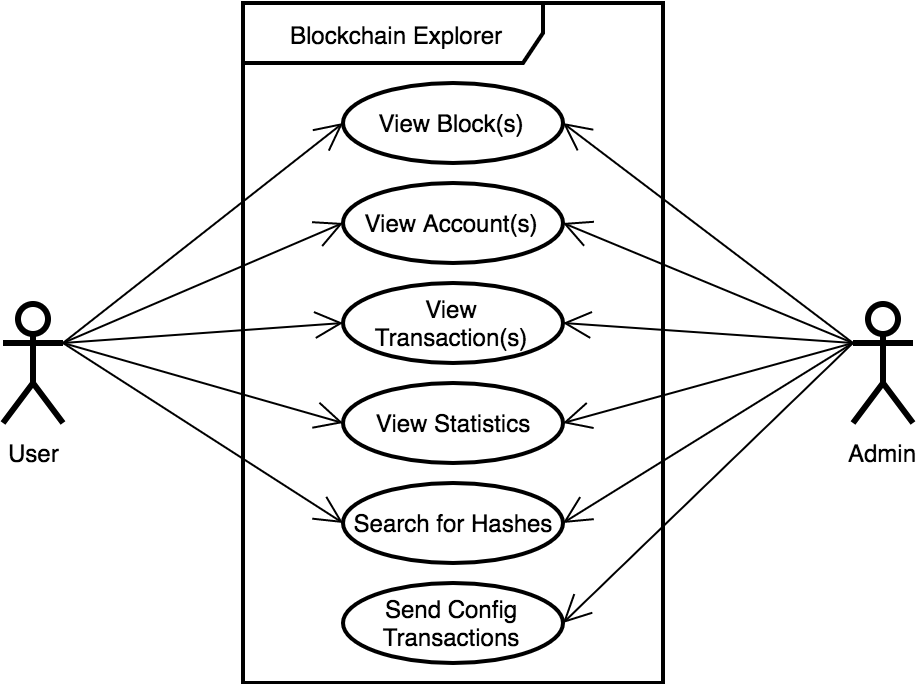
\includegraphics[scale=0.35]{usecase1.png}
  \centering
  \caption{Use Cases of the Block Explorer}
  \label{fig:usecase1}
\end{figure}

\begin{itemize}
\item \textbf{Blocks}\\
A user should be able to view all validated blocks of the blockchain and the information they contain. In a list-view, the most recent blocks are being displayed, identified by their respective hashes and timestamps. If a user wants to get more comprehensive information about a block, he can display one block in a detailed-view, where additional information, such as all the transaction hashes contained in this block or the address hash of the block-reward beneficiary are presented.
\item \textbf{Transactions}\\
Similarly to the requirement above, a user should be able to view all validated transactions that have been broadcasted by him or other users of the blockchain. Due to the Bazo system having 4 different types of transactions (Funds Transactions, Account Creation Transactions and System Configuration Transactions from the original Bazo paper \cite{bazo} and Stake Transactions from the Proof-of-Stake implementation \cite{pos}), different implementations for each of them have to be made. A list-view displays the most recent transactions of each type, offering information such as the sender, receiver and the amount of the transactions. Detailed views for all transaction types are needed as well, presenting more information, for example each transaction's signature or block it is contained in.
\item \textbf{Accounts}\\
With Bazo using an account-based model, every user that actively interacts with the blockchain owns an account. The application should maintain a state of all accounts, that gets updated with every newly mined block. A list with the most affluent accounts should be made available, as well as a detailed view of for single accounts, which displays all transactions this account was either the sender or receiver of.
\item \textbf{Search}\\
A user should be able to search for blockchain data using hashes. These hashes can be identifiers of blocks, transactions or accounts, with accounts having both addresses and address-hashes. A user should not need to choose what he actually searches for, meaning the application searches through all data it has collected and, in case of a hit presents the data associated with the hash to the user, and in case of a miss, notifies the user of not finding any relevant data.
\item \textbf{Navbar}\\
Featured on every page of the application, a navbar, that lets a user access all functionality of the website, is required. This functionality includes, among others, links to lists of blocks, transactions and accounts. The search-functionality is also located here, being available at all times to the user.
\item \textbf{Statistical Information}
The system should calculate statistical information about the network and make it available to users. This includes information such as a graphical history of transactions, or the total amount of Bazo Coins currently in the system.
\item \textbf{Administrator Panel}\\
Only available to admins of the system, a panel that lets them change system parameters using System Configuration Transactions has to be implemented. These transactions get sent via an interface \cite{marc} to the network, meaning no Bazo Client is running on the server of the website.
\item \textbf{Fetch and Store Blockchain Data}\\
The application needs to automatically gather the latest Bazo Blockchain data and save it independently from the blockchain. This data also needs to be correctly formatted, in order to make it accessible to the users. 
\end{itemize}

\section{Structure of the Service} \label{structure}
The main component of the Bazo Blockchain Explorer that users and admins use to view Bazo Blockchain data is a web app, which is made up of a front- and a backend. However, to run the blockchain explorer on its own, additional components beside the front- and backend components are required. Highlighted in red in Figure \ref{fig:structure} are the components that were implemented as part of this thesis. The backend fetches blockchain data from a database that runs independently from the blockchain miner's built-in storage. A separate database was chosen, because additional data like statistical information needs to be calculated and stored as well, which would bloat all miner's built-in databases with information, if implemented in the miner. This also makes running the website possible without having a miner running in the backend of the web app. However, this requires a component that copies data from a running Bazo mining node's storage and stores it in the new database. As mentioned above, the web app's backend accesses this database by making queries for relevant data and sending the results to the frontend to be displayed to the user. In order to fulfil the requirement of being able to send System Configuration Transactions from the application, an interface that acts as an extension for a Bazo Client is required. With the use of this interface, signing transactions without a running Bazo Client will be made possible.

\begin{figure}[h]
  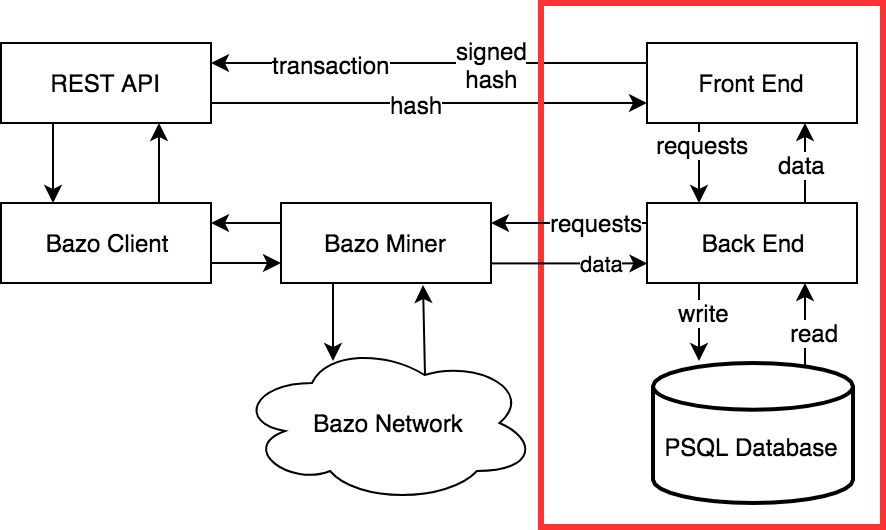
\includegraphics[scale=0.4]{system.png}
  \centering
  \caption{Structure of the Blockexplorer and Bazo Components}
  \label{fig:structure}
\end{figure}

\subsection{Trust}
The operator of the blockchain hosts the system, which in this case is connected to a miner that also belongs to the operator. Due to the open-source nature of the block explorer however, anyone can run and host a Bazo Blockchain Explorer on his or her servers and connect to a miner of choice. A discussion about whether the miners, to which the explorer connects, need to be trusted or not, is not required, since (1) the operator has no interest in presenting its users falsified data, (2) in case doubt arises about the data's authenticity, anyone can host his own explorer, and (3) from a user's perspective, the explorer only \emph{consumes} data from the blockchain. The running Bazo blockchain is therefore not affected by any block explorers.

\section{Web Application}
A web application was chosen, because of its accessibility and its convenience. Users do not need to download software or store data on their devices to inspect the blockchain. The user interface of the application always displays the most recent blockchain data.  In order to structurally separate the functionality and to fulfil all requirements, specific pages featuring the following content need to be included in the application:

\begin{itemize}
\item{List of Most Recent Blocks}
\item{Detailed Block}
\item{List of Most Recent Funds Transactions}
\item{Detailed Funds Transaction}
\item{List of Most Recent Account Creation Transactions}
\item{Detailed Account Creation Transaction}
\item{List of Most Recent Configuration Transaction}
\item{Detailed Configuration Transaction}
\item{List of Most Affluent Accounts}
\item{Detailed Account}
\item{Statistical Information}
\item{Administrator Panel}
\end{itemize}

\begin{figure}
  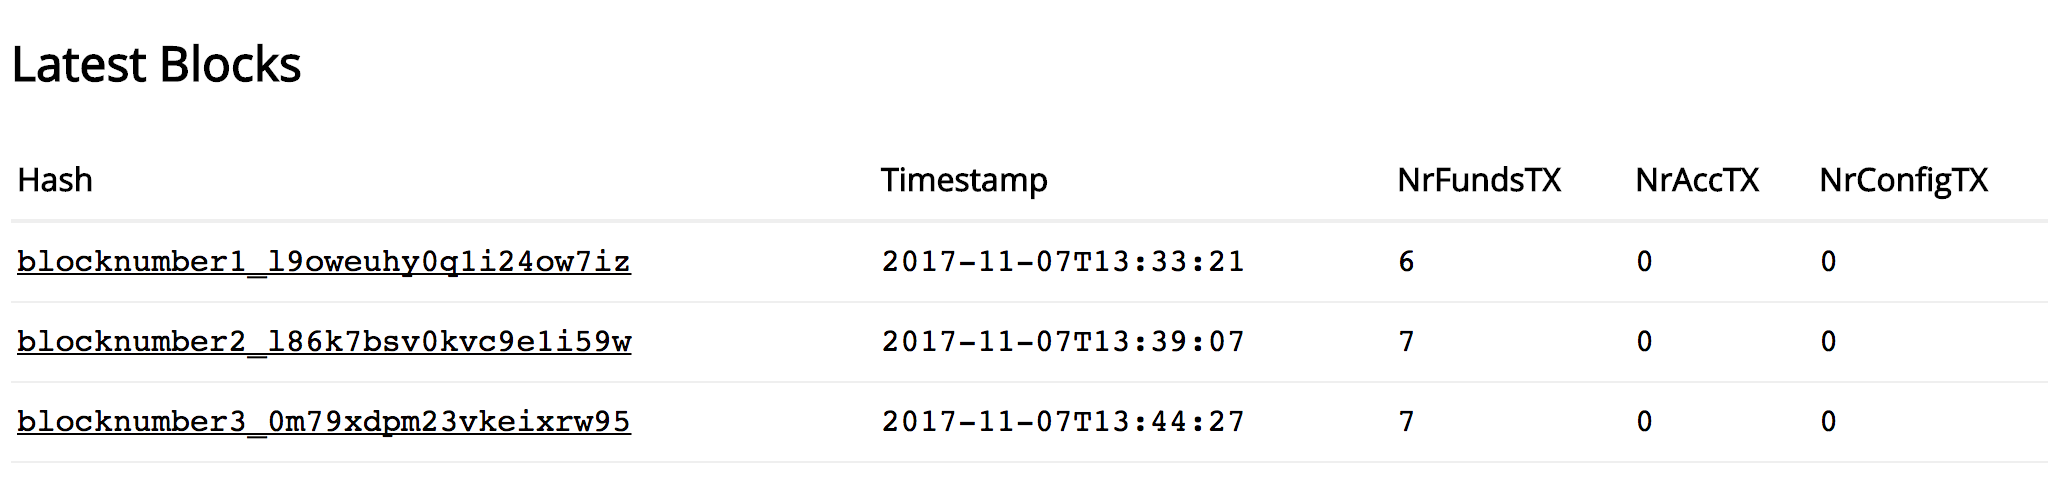
\includegraphics[width=\linewidth]{mockup1.png}
  \centering
  \caption{Mockup of the List of Most Recent Blocks}
  \label{fig:mockup1}
\end{figure}

From a list-view of a data-type, each individual item can be accessed. The goal is to first, provide the user with a list view of a data-type, such as blocks. Once he finds an object of interest, he clicks on the hash of the block, which is its unique identifier, and gets presented with detailed information about that object. Depending on the data-type, the user is viewing, links to related elements enable further browsing of the data. For example, on a detailed block page, a link to the detailed account page of the account that received the block reward of said block, is listed. Since all different types of blockchain data have their own data structures, custom tables for all listed pages, that contain data need to be built. In Figure \ref{fig:mockup1}, a mockup of the table containing the most recent blocks is displayed. The block's hash, the timestamp when it was mined and the counters for each transaction type are listed. Each single block hash links to the detailed page of that block. On the detailed block page, all transaction hashes that are included in a block, are ordered by type and displayed in a list. Similarly on a detailed account's page, all transactions related to that account are displayed as well.

\subsection{Navbar and Search}
The navbar is featured on every page of the application. Figure \ref{fig:navbar} displays all possible pages that are accessible from the navbar and the their respective detailed pages. Since there are multiple types of transactions, a dropdown menu on the \emph{Transactions} button, displays links to list-views of all types of transactions. The administrator panel is also accessed from here. Included in the navbar, is the search function. A user can enter a hash and the backend of the application searches for that hash in the database. A successful search will automatically present the data to the user in the right formatting, meaning the system displays the page according to the data type of the search result. It is possible to search for blocks, all transaction types, account hashes and account addresses, since Bazo uses both hashes and addresses to identify an account.

\begin{figure}[h]
  
\includegraphics[scale=0.35]{navbarmockup.png}
  \centering
  \caption{Functionality and Links on the Navbar}
  \label{fig:navbar}
\end{figure}

\subsection{URL-Scheme}
Keeping URLs as simple as possible was a priority. Since a specific object may only be identified by its hash or its address, either is the only variable that is needed in a URL for specific objects. In the following frame, sample URLs and the pages they display are presented. The segment \emph{host} is a placeholder for the domain, the block explorer is hosted on.

\begin{framed}
\url{host/blocks} --- List of most recent blocks

\url{host/block/<<block_hash>>} --- Details for block $\ll$blockhash$\gg$

\url{host/adminpanel} --- Administrator panel

\url{host/tx/funds/<<hash>>} --- Details for Funds Transaction $\ll$hash$\gg$

\url{host/tx/acc} --- List of most recent Account Creation Transactions
\end{framed}

\subsection{Administrator Panel}
Since there currently are five different types of System Configuration Transactions defined by IDs 1 through 5 \cite{bazo}, a \emph{Submit} form for every type needs to be available on the administrator panel. Depending on which administrator is currently logged in and using the panel, account information, such as the current transaction count and public key of the administrator, do not need to be entered in the transaction forms. These values get automatically included in the transactions are are derived from the public key, the administrator entered to log in. Detailed information about the verification process can be found in Section \ref{cookies}. The administrator enters the payload for the transaction he wishes to send and the transaction fee. The application validates the user input before sending transaction details. The panel also displays all current system parameters and updates them after each validated System Configuration Transaction. 

\subsection{Statistical Information}
On this section of the application, users can view data about the overall health and productivity of the Bazo blockchain. A chart featuring a 12-Hour transaction history visualizes how frequently the Bazo system is used, as well as shows, whether usage increases over time of operation. Information regarding total Bazo Coin supply and the total number of Bazo accounts is also provided, since viewing accounts and their balances by all users, is possible anyway. The statistical information is updated in a regular interval, to match the recent blockchain data.

\section{Database}
A relational database was chosen for the Bazo Block Explorer, because the data the explorer uses, is always structured in the same format. Blocks and transactions have attributes defined in the Bazo protocol, which were carried over for use in the database. Using tables, the data can be sorted efficiently by attributes like timestamps or transaction amounts, due to the flexibility of SQL queries. The Bazo protocol uses BoltDB \cite{bolt} in its Miner program, which is a key/value based store, where the hash, a unique identifier, represents the key and encoded block or transaction information represents the value.
When users perform a search on the web app, they exclusively search for hashes, unique to each object. This enables defining the hashes as primary keys in the tables. However, the database performs additional queries using that hash. For example, when a user searches for an account, the system also queries the Funds Transaction table with the same hash to look for all transactions that account was a part of. This also speaks for using SQL queries. 

As mentioned in Section \ref{structure}, additional information regarding the blockchain data needs to be calculated and stored, so additional tables for statistical data need to be defined and maintained. For optimal performance the database is hosted on the same server as the block explorer, to ensure efficient read or write times. The statistical data also needs to be calculated either in a fixed interval or after a certain event has happened.

\subsection{Tables}
The following tables and attributes need to be defined to accommodate all Bazo objects and data. Where needed, indexes have been added to increase performance. Primary keys are underlined, while indexes are in italics.
\begin{itemize}
\item \textbf{Blocks}
Header, \underline{\textit{Hash}}, PreviousHash, Nonce, \textit{Timestamp}, Timestring, MerkleRoot, Beneficiary, NrFundsTx, NrAccTx, NrConfigTx, FundsTxData, AccTxData,\\ ConfigTxData
\item \textbf{Accounts}
 \underline{\textit{Hash}}, \textit{Address}, Balance, TxCount
\item \textbf{Funds Transactions}
Header, \underline{\textit{Hash}}, BlockHash, Amount, Fee, TxCount, \textit{Sender}, Recipient, Timestamp, Signature
\item \textbf{Account Creation Transactions}
Header, \underline{\textit{Hash}}, BlockHash, Issuer, Fee,\\ PublicKey, Timestamp, Signature
\item \textbf{System Configuration Transactions}
Header, \underline{\textit{Hash}}, BlockHash, Id, Payload, Fee, TxCount, Timestamp, Signature
\item \textbf{Parameters}
Timestamp, BlockSize, DifficultyInterval, MinimumFee,\\ BlockInterval, BlockReward
\item \textbf{Stats}
TotalSupply, NrAccounts, Timestamp
\end{itemize}

\chapter{Implementation}
This chapter documents the structuring and implementation of the components listed in Chapter \ref{chap:design} and how they interact with each other. An additional section concerning hosting of the application on the internet is also included. The majority of the application was programmed in Go (Golang to avoid confusion). Go is a language that started development in 2007, as an answer to the changing computer landscape, as no new major systems language has emerged over a long time \cite{gohistory}. The aim of Go is to support new computing concepts such as multicore computing and make development overall a less time consuming task.

\section{Packages of the Block Explorer}
The backend of the web app is written in Golang \cite{golang}, which is well suited for writing web applications, due to its included net/http \cite{httppackage} and html/template \cite{template} packages. Since the Bazo Blockchain was also written in Golang \cite{bazo}, compatibility between the two programs was ensured and certain packages of Bazo were used in the Bazo Block Explorer. The program is split up into distinct modules, to separate functionality. Dependencies are presented in Figure \ref{fig:packages} \\ \\

\begin{figure}[h]
  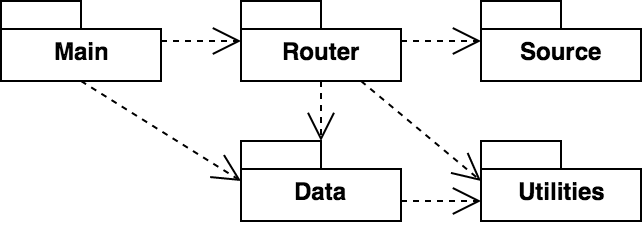
\includegraphics[scale=0.4]{packagesnew.png}
  \centering
  \caption{Package-Diagram of the Blockchain Explorer}
  \label{fig:packages}
\end{figure}

\begin{itemize}
\item \textbf{Router}\\
The Router functionality is described in Section \ref{router}. It handles all requests made to the application, from the browser. The appropriate data is then loaded and sent in response.
\item \textbf{Data}\\
This module handles all data processing of the application, specifically the retrieval of data from the blockchain and the saving of that data in the block explorer's own database. It is described in Section \ref{data} and Section \ref{sql}.
\item \textbf{Utilities}\\
The Utilities module contains functionality that is used by both Router and Data modules such as the definition of structs, handling of cookies and smaller helper functions.
\item \textbf{Source}\\
All Gohtml templates, JavaScript files and CSS files are contained in this module. Gohtml templates get passed to the router, which then get converted to HTML, whereas the other files get served to the website to be used client-side.
\end{itemize}

\section{HTML Templates}
To interact with the Golang-Backend of the application, Gohtml templates \cite{template} have been used to define the markup of the pages. One one hand, this makes way for a modular view component by letting programmers define reusable HTML modules such as headers, footers or table-templates. Using templates can minimize code duplication, which in turn makes maintenance on the code an overall less risky task. On the other hand, Golang templates allow for some limited logic in the Gohtml files, which is needed for handling variables that get passed from the backend component. For example, if the passed variable is an array of integers and the goal is to display all variables in a list, golang can create a new <li> tag for every value in the array. The HTML code that gets passed to the end user after making a request contains no Golang code, since the backend renders the Gohtml template files and passed variables to a useable HTML file that can be displayed by a web browser \cite{httppackage}. Except for the rendering of the chart on the statistical information page mentioned in Subsection \ref{chart} and one special case discussed in Subsection \ref{vuejs}, all rendered pages of the application are static HTML files, because for every action a user may make on the website, a request has to be made to the backend. The website aims to always display the most recent data, so storing information that may not be up to date on the client's machine in order to save bandwidth, is outweighed by the possibility of having more recent data. To appropriately handle relative paths on the templates, a \emph{UrlLevel} string depending on the current URL, for example ``../", is always passed to the template, in addition to the regular blockchain data. This string is prepended dynamically to all links in the navbar, so that the same templates can be used on different URLs.

\subsection{Reusable Modules}
\begin{itemize}
\item \textbf{Navbar}\\
Since the Navbar is featured on every page of the explorer, it was defined as a reusable template.
\item \textbf{HTML Head}\\
Every page features the same links to stylesheets and meta information. Thus the content of the HTML Head is reusable.
\item \textbf{Public Key Modal}\\
The modal that expects a public key to authenticate a user, is accessible from the navbar and therefore can be defined as a template.
\item \textbf{Private Key Modal}\\
For sending transactions from the admin panel, a modal that expects an administrator's private key is derived from the login modal and kept as a template.
\item \textbf{Script Imports}\\
For JavaScript functionality, a group of \emph{script} tags have been pooled, similarly to the HTML head's imports.
\end{itemize}

\subsection{Handling Passed Variables}
If the backend of the application passes any variable to a template, Gohtml templates can render these variables by including ``\{\{ . \}\}'' in the template. Golang code is delimited by curly braces inside templates. The period is the placeholder, the passed variable replaces, before being rendered to HTML. When passing a struct to a template, all attributes of the struct can be accessed, by appending the attribute name to the period. In order to pass different structs to the template, such as in the landing page's case, where slices of blocks \emph{and} slices of transactions are passed, structs containing structs need to be defined, since only one object can be passed to the template. 

In Listing \ref{lst:structtable}, a simplified excerpt from the landing page Gohtml file is presented. Two tables, one for block-hashes and one for Funds Transaction hashes make use of templating. A struct containing a slice of blocks and a slice of Funds Transactions, gets passed to the template. On line 8, the \emph{Blocks} slice (attribute) of the passed struct gets iterated through using the \emph{range} and \emph{end} keywords. For every block, a new table row gets created, containing a link to the specific block page. The period now represents the struct of a single block and its attributes can be accessed by appending the desired attribute. Similarly on line 23, the transaction slice in the struct is iterated through. On line 25, the \emph{Hash} attribute does not access the block's hash anymore, but the Funds Transaction's, as the period now represents a transaction.
\newpage
%\begin{minipage}{\linewidth}
\begin{lstlisting}[caption={Block and Funds Transaction Tables Accessing a \emph{blocksandtx} Struct},captionpos=b,label={lst:structtable}]
<table class="table">
  <thead>
    <tr id="header-row">
      <th>Hash</th>
    </tr>
  </thead>
  <tbody>
    {{range .Blocks}}
    <tr>
      <td><a href="block/{{.Hash}}">{{.Hash}}</a></td>
    </tr>
    {{end}}
  </tbody>
</table>

<table class="table">
  <thead>
    <tr id="header-row">
      <th>Hash</th>
    </tr>
  </thead>
  <tbody>
    {{range .Txs}}
    <tr>
      <td><a href="tx/funds/{{.Hash}}">{{.Hash}}</a></td>
    </tr>
    {{end}}
  </tbody>
</table>
\end{lstlisting}
%\end{minipage}

\section{UI Framework} \label{sec:uiframeworks}
In the beginning of development, a custom CSS built from scratch was created to style the application, however, due to concerns about usability and overall presentation of the website, the Bootstrap v4 UI Framework \cite{bootstrap} was chosen as a replacement and enhancement of the original styling.
``Originally created by a designer and a developer at Twitter, Bootstrap has become one of the most popular front-end frameworks and open source projects in the world.'' \cite{bootstraphistory}
It offers a wide variety of content and components to quickly build a responsive user interface. Most components are defined in the Bootstrap CSS, however for some client-side functionality, JavaScript can be enabled. Block explorer pages are heavily dependent on Bootstrap, since all UI components use Bootstrap classes. In cases where further styling was needed, a separate CSS overwrites Bootstrap stylings, for example the width of the Search Bar had to be manually widened. In some tables, inline styling in their HTML was used, when certain columns needed to have fixed widths. Figure \ref{fig:landing} presents the landing page of the block explorer, featuring Bootstrap components.

\begin{figure}
  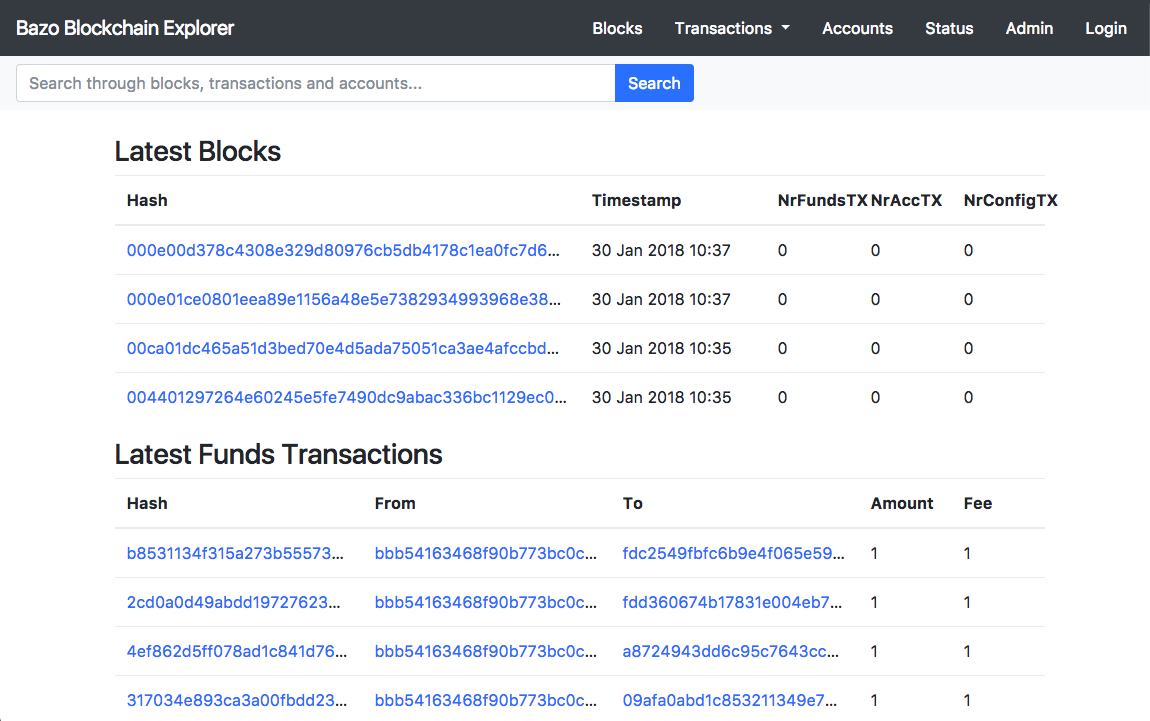
\includegraphics[scale=0.35]{landingpage.png}
  \centering
  \caption{Landing Page of the Explorer}
  \label{fig:landing}
\end{figure}

\section{Client-Side Logic} \label{sec:clientside}
The explorer uses a JavaScript \cite{javascript} framework and different libraries to implement client-side logic, which was used to implement the sending of transactions and the rendering of a chart.
\subsection{Vue.js and Libraries} \label{vuejs}
For the process described in subsection \ref{txsigning}, the Vue.js JavaScript framework \cite{vue} is used. Vue.js allows for easy client-side scripting with minimal setup. It links a vue app which is contained in a JavaScript file to an \emph{id}-tag on a HTML file and has access to all objects such as input fields and buttons under the \emph{div}-tag that contains the linked  \emph{id}-tag. To run a vue app, vue and all the additional libraries have to be imported on the HTML file. Additionally to the standard vue import, Axios , a promise based HTTP client \cite{axios} has been used to make GET requests from the frontend of the application. To extract cookies for verification purposes, vue-cookies \cite{vcookies} was used. 

\subsection{Transaction Signing} \label{txsigning}
A requirement of the Bazo Blockchain Explorer is to be able to send System Configuration Transactions from the browser. 
However, since no Bazo Client should run in the backend of the application, the ability to build and sign transactions is not provided. A Bazo Client takes transaction details and the private key of the sender in order to build a transaction. Extracting only the transaction signing functionality of the Bazo Client and implementing it into the backend of the explorer would violate security constraints, since the private key would have to be sent over the network to the server. The private key should always stay with the user and never leave his device. This is where the Bazo Interface \cite{marc} comes in place, a REST API that builds an unfinished transaction hash using the transaction details without the issuer's private key. In a second step the user enters his private key in order to sign the transaction client-side and then send it back to the Interface, which then publishes it to the network.

\begin{figure}
  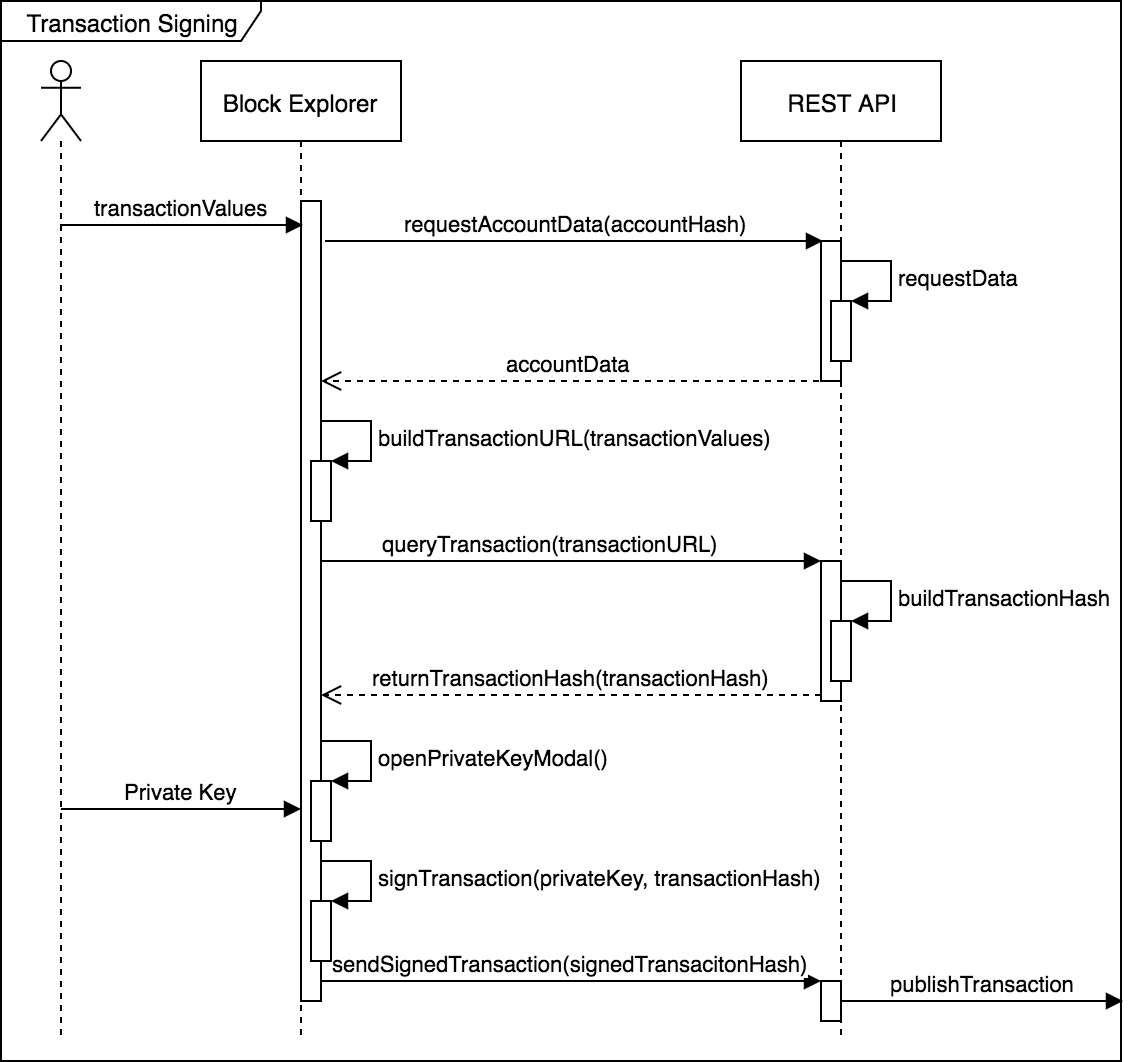
\includegraphics[scale=0.35]{transactionbuilding.png}
  \centering
  \caption{Sequence Diagram of How the Application Builds and Signs Transactions}
  \label{fig:sequence1}
\end{figure}

The process is detailed in Figure \ref{fig:sequence1}. A user enters the values that make up the transaction into HTML-input fields on the administrator panel, which are linked to a Vue.js application \cite{vue} . In this case, that would be the type of Configuration Transaction (id), the payload (new value) and the transaction fee. When the user hits \emph{Send}, JavaScript code in the Vue.js app extracts the public key stored in a cookie \cite{vcookies} (user verification is described in Section \ref{cookies}) and requests the account data concerning that user. The REST interface responds with the account information in JSON format \cite{json}, of which the \emph{isRoot} attribute is important to the application. If the public key, stored in the cookie belongs to a root account, the JavaScript code builds a URL that contains all transaction data, previously entered by the user. Another request to the interface, using that URL is made, which then builds a transaction hash using the transaction data. If that hash was returned successfully, a modal opens up on the block explorer, prompting the user to enter a root private key. Using a JavaScript implementation of elliptic signing \cite{elliptic}, the transaction hash gets signed with the entered private key, which results in a new, signed transaction hash and sent to the interface, along with the unsigned hash for identification purposes.

\subsection{AnyChart} \label{chart}
To render the chart that displays the 12-hour transaction history of the network, the AnyChart JavaScript charting library \cite{anychart} was used. It allows the creation of over 70 different charts and the only thing it requires the backend to do, is format the data in the correct way. On the HTML-template, script imports can be used to make use of the library, which makes the use of a packet manager unnecessary. In addition to imports, it requires a JavaScript function, that defines the type, layout and the location of the diagram on the final page. The location is defined by an HTML \emph{id} tag. In the Bazo Block Explorer's case, a spline chart was chosen to display the data in a line.
The backend requests all blocks that were mined in the last 12 hours, calculates the total number of transactions for each hour and saves that information in a struct. That struct gets converted into JSON format and then converted to a string. This string then gets passed to the template and used by the AnyChart function, which converts the string back to JSON format and uses it to build the chart.

\section{Router} \label{router}
The router handles all requests made to the application. The process of initializing the router is detailed in Listing \ref{lst:router}. When \emph{InitializeRouter()} is called, a new router is declared and registers all possible routes to it. Furthermore, all Gohtml templates and JavaScript files are passed to the router, so they can be rendered and used upon request \cite{httppackage}. 
Additionally to the built-in http package in Golang, HttpRouter by Julien Schmidt \cite{httprouter} has been used. 
``In contrast to the default mux of Go's net/http package, this router supports variables in the routing pattern and matches against the request method. It also scales better.'' \cite{httprouter}
HttpRouter makes building a routing table convenient. All routes and the functions they invoke, once called, can be defined in a well-structured way. Variables in the routes such as hashes can be defined by prepending a colon before a segment in the URL. For example in listing \ref{lst:router} on line 6, when \emph{/blocks/:hash} is called using a GET request, where \emph{:hash} can be any string variable, the router automatically parses the hash to be used by the \emph{getOneBlock()} function that gets called after the request. Except for the \emph{/login} and \emph{/search} routes, which are called using POST methods, all routes are called via GET request.
\newpage
%\begin{minipage}{\linewidth}
\begin{lstlisting}[caption={Initialization of the Router},captionpos=b,label={lst:router}]
func InitializeRouter() *httprouter.Router {
  tpl = template.Must(template.ParseGlob("source/html/*"))
  router := httprouter.New()

  router.GET("/", getIndex)
  router.GET("/blocks", getAllBlocks)
  router.GET("/block/:hash", getOneBlock)
  router.GET("/tx/funds", getAllFundsTx)
  router.GET("/tx/funds/:hash", getOneFundsTx)
  router.GET("/tx/acc", getAllAccTx)
  router.GET("/tx/acc/:hash", getOneAccTx)
  router.GET("/tx/config", getAllConfigTx)
  router.GET("/tx/config/:hash", getOneConfigTx)
  router.GET("/account/:hash", getAccount)
  router.GET("/accounts", getTopAccounts)
  router.GET("/stats", getStats)
  router.POST("/search", searchForHash)
  router.POST("/login", loginFunc)
  router.GET("/logout", logoutFunc)
  router.GET("/adminpanel", adminfunc)

  router.ServeFiles("/source/*filepath", http.Dir("source"))

  return router
}
\end{lstlisting}
%\end{minipage}

\section{Cookies} \label{cookies}

By design, only administrators of the system can successfully publish a System Configuration Transaction to the network, since only they possess a root private key that lets them sign the transactions. However, using a Bazo Client, a non-root user may still spam the network with admin-only transactions, without them ever getting accepted by the system. Therefore implementing a thorough login-system on the explorer that requests a user's private key to verify whether he has administrator rights, in order to prevent non-administrator users from trying to publish transactions to the network seemed unnecessary. This would have also meant that a private key would get sent over the network to check its access rights. The chosen verification process is as follows:
Upon requesting to log in, a modal appears, where a user is requested to enter his \emph{public} key. The modal is presented in Figure \ref{fig:login}. This public key then gets sent to the Bazo Interface \cite{marc}, where more information regarding that key is requested. One attribute of the response the interface returns, is \emph{isRoot}. If \emph{isRoot} returns true, a cookie containing the entered public key gets saved to the user's machine and the user is verified. When the user then requests the administrator panel, the only page requiring verification, the public key in the cookie gets checked again and sent to the interface. If the returned \emph{isRoot} is still true, he gets access to the administrator panel. The public key contained in the cookie then gets extracted by client-side code described in Section \ref{txsigning} when the process of sending a Configuration Transaction is initiated.

\begin{figure}
  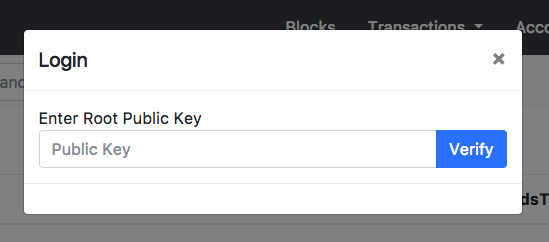
\includegraphics[scale=0.5]{loginmodal.png}
  \centering
  \caption{Login Modal Requesting the User's Public Key}
  \label{fig:login}
\end{figure}

\section{Concurrency} \label{goroutines}
The application makes use of Golang's built-in concurrency functionality. By calling \emph{runDB()} in the main function as a Goroutine by prepending the keyword \emph{go}, the mechanism that automatically updates the database with new blockchain data, runs separately from the router's request handling. This means that the web app can still be used, while the database is being updated with new records.

\section{Structs}
Hashes and other generated values in the Bazo blockchain are stored using fixed-sized byte-slices. This has several drawbacks in terms of usability, since they first have to be converted into strings by representing each byte in its hexadecimal value and concatenating all hex values, when displayed to the user. Because of difficulty preserving the byte-slices while storing them in a PSQL database, and the fact that users search for string representations of these values, all blockchain data first gets converted to human-readable form before saving it in the database. Additionally for easier data-management, all entries in all transaction tables now have added \emph{BlockHash} and \emph{Timestamp} attributes, since using raw blockchain data, transactions could not be traced back to a block, a mining date, or a transaction time. The struct definition of an Account Creation Transaction in the explorer can be seen in Listing \ref{lst:acctxstruct}

\begin{lstlisting}[caption={Struct Definition of an Account Cration Transaction},captionpos=b,label={lst:acctxstruct}]
type Acctx struct {
  Hash string
  BlockHash string
  Issuer string
  Fee uint64
  PubKey string
  Timestamp int64
  Signature string
  UrlLevel string
}
\end{lstlisting}
\section{Data Transfer} \label{data}
This section explains how blockchain data is retrieved from a node and stored. After requesting the block-data, the block extracts transaction information to make additional requests for transaction data. All retrieved information is then stored in the database.
\subsection{Retrieving Blocks} \label{retrieve}
When \emph{runDB()} is called as a Goroutine, as mentioned in Section \ref{goroutines}, all existing blocks are requested from the blockchain and stored in the database. To request a block and its data, the blocks's hash needs to be known. Integrated into the miner is the functionality that, if a block is requested but \emph{nil} is passed to the function, the most recent block in the miner's storage component (known as \emph{newestBlock}) is returned and subsequently saved to the explorer's database. Starting with this  \emph{newestBlock}'s \emph{previousHash} attribute, the remaining blocks get requested and saved recursively until the genesis block is reached. Once all existing blocks have been saved, the system regularly checks whether there have been any new blocks mined and retrieves them in a similar fashion.
The way a block is requested is similar to how Bazo Miners communicate with each other \cite{bazo}. The application imports the miner's p2p package and utilizes its messaging system to connect to the bootstrap server and make requests to the network.

\subsection{Procedure for Saving a Block} \

%\begin{minipage}{\linewidth}
\begin{lstlisting}[caption={Saving a Block and Its Transactions to the Database},captionpos=b,label={lst:save}]
func SaveBlockAndTransactions(oneBlock *protocol.Block)  {

  for _, accTxHash := range oneBlock.AccTxData{ . . . }

  for _, fundsTxHash := range oneBlock.FundsTxData{
    fundsTx := reqTx(p2p.FUNDSTX_REQ, fundsTxHash)
    convertedTx := ConvertFundsTransaction(fundsTx.(*protocol.FundsTx), 
    										oneBlock.Hash, 
											fundsTxHash)

    UpdateAccountData(convertedTx)
    WriteFundsTx(convertedTx)
  }

  for _, configTxHash := range oneBlock.ConfigTxData{ . . . }

  convertedBlock := ConvertBlock(oneBlock)
  WriteBlock(convertedBlock)
}
\end{lstlisting}
%\end{minipage}

Every block retrieved from the miner goes through the algorithm presented in Listing \ref{lst:save}. Since every block contains a slice of transaction hashes for every transaction type, loops that iterate through the slices exist for every transaction type (lines 3, 5 and 15). Account Creation Transactions and Configuration Transactions have been minimized in the example, to highlight how Funds Transactions are saved in the database. All processes are similar and only differ in what information is saved and updated in their respective tables.

Starting on line 5, a request using the Funds Transaction's hash, to retrieve the full transaction data is made to the network. The returned transaction of type \emph{protocol.FundsTx} is then converted to a struct that is usable to the database. For the conversion, the block's hash and the transaction hash, extracted from the slice, are needed as well. \emph{UpdateAccountData(convertedTx)} then updates \emph{Balance} and \emph{TxCount} attributes for all accounts featured in that transaction in the database's \emph{Accounts} table. The last step concerning the transaction is \emph{WriteFundsTx(convertedTx)}, which saves the transaction in the \emph{FundsTx} table in the database. After all slices have finished processing, the block itself is converted to a database-friendly format and saved in the \emph{Blocks} table.

\section{SQL-Queries} \label{sql}
On startup, the first database queries made, are called from the \emph{DBSetup()} function. First, all existing tables and data get dropped from the database. Then, all tables get created again to start the application with a clean database. Once the explorer begins requesting and saving blocks from the network, \emph{INSERT} queries begin writing all data in their respective tables, block by block. \emph{SELECT} statements are used when requesting one or more rows of data from a table. Using Golang's \emph{database/sql} package, placeholder values, such as \$1, \$2, etc an be used to automate construction of the SQL-Statement string. The actual variables can be passed as additional arguments to the function that is used to query the request, as seen in Listing \ref{lst:acctx}: \emph{UrlHash} represents the hash, the user has requested. Together with the statement string, it gets passed to \emph{db.QueryRow} and saved to \emph{row}. The next step is mapping all values of  \emph{row} to a struct that matches all columns of the query result using the \emph{Scan()} function of the \emph{row} object. Additionally to write and read functions for blocks, transactions and accounts, functions that update and return the statistical information also exist.
\\
\begin{lstlisting}[caption={Requesting a Specific Account Creation Transaction},captionpos=b,label={lst:acctx}]
sqlStatement := `SELECT hash, blockhash, issuer, fee, pubkey, signature 
				 FROM acctx 
				 WHERE hash = $1;`
row := db.QueryRow(sqlStatement, UrlHash)
var returnedrow acctx
row.Scan(&returnedrow.Hash, &returnedrow.BlockHash, &returnedrow.Issuer,
		 &returnedrow.Fee, &returnedrow.PubKey, &returnedrow.Signature)
\end{lstlisting}

\subsection{Search Function}
When a user enters a hash he wants more information on, it gets passed to the backend and processed by the \emph{searchForHash} function, which makes a request with the entered hash on each table, until a table returns a result. If no data regarding that hash could be found, the user is notified.

\section{Hosting}
In a test-run, the Bazo Block Explorer was hosted as a Heroku app on their cloud hosting platform \cite{heroku}. The PSQL database was also ported to run on Heroku. Since during development, both the explorer and the database were hosted locally, changes to how the application retrieves the target port and database connection string needed to be made. On Heroku, the application and the database were connected by adding the database as an add-on to the Heroku App. This means that the correct port and database location can be extracted using Golang's \emph{os} package \cite{os}. These values can also be edited manually using Heroku's dashboard.

Required for the Golang application to compile and run on Heroku, is the \emph{heroku/go} buildpack \cite{buildpack}, which is used to install dependencies and configure the environment. Additionally the application needs a procfile, which specifies how Heroku will name and treat the application \cite{procfile}. In the block explorer's case it was defined as a \emph{web} app.
\begin{framed}
web: BlockExplorerHeroku
\end{framed}
Godep needs to be used to manage dependencies of the app \cite{godep}. Godep saves all dependencies in JSON \cite{json} format, which are then interpreted by the \emph{heroku/go} buildpack \cite{buildpack}. When the application is pushed to heroku, it gets built using all dependencies and is useable immediately.
